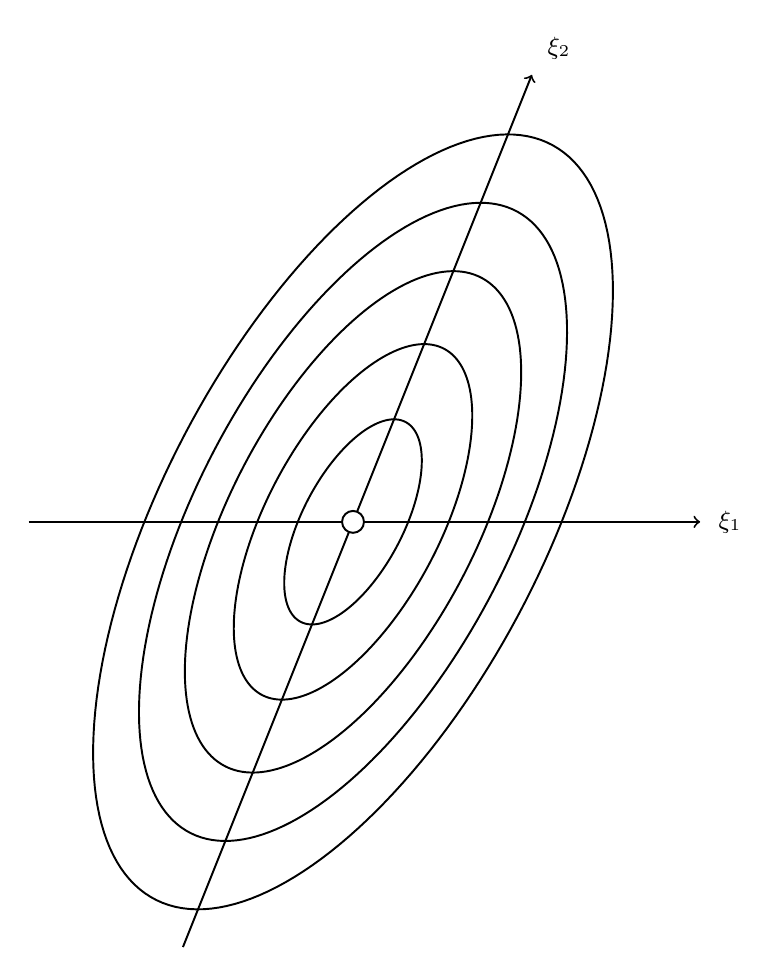
\begin{tikzpicture}[scale=2.4742,font=\small,x=0.9cm,y=0.9cm,line width=0.7pt]
  % Affine image of u'=-v, v'=u under P=[(0.70,0)^T,(0.52,1.30)^T].
  % The source shows closed orbits without flow arrows.
  \foreach \r in {0.45,0.78,1.10,1.40,1.70} {
    \draw plot[domain=0:360,samples=180,variable=\a]
      ({\r*(0.70*cos(\a)+0.52*sin(\a))},{1.30*\r*sin(\a)})--cycle;
  }
  \draw[->] (-1.85,0)--(1.98,0);
  \draw[->] (-0.97,-2.425)--(1.02,2.55);
  \fill[white] (0,0) circle (1.6pt);
  \draw (0,0) circle (1.6pt);
  \node[right=3pt] at (1.98,0) {$\xi_1$};
  \node[above right=2pt] at (1.02,2.55) {$\xi_2$};
\end{tikzpicture}
